%% ----- INTRODUCTION -----
\hypertarget{server-experiments-introduction}{%
\section{Introduction}\label{server-experiments-intro}}

Before my arrival at TU Berlin's department of Transport Planning and Transport Telematics, known by its German acronym \gls{VSP}, I amassed two decades of software development experience at the intersection of transport modeling and user interface design. This combination led to some interesting and novel research, such as the CycleTracks bicycle route choice model and mobile-phone based data collection approach described in \cite{HoodSallCharlton2011BicycleRouteChoiceSanFrancisco}, the QuickMuni transit-arrival app\footnote{QuickMuni, available at \url{https://billyc.github.io/quicky/}}, and the San Francisco County Transportation Authority ``TNCs Today'' data exploration web portal described in \cite{erhardt2019transportation}.

At VSP, these projects triggered interest in developing web-based visualizations for MATSim outputs. We set out to adapt some of the technologies used in the efforts listed above. Initially there was no end goal in mind: this was pure research to ascertain how far we could go with web-based technologies. Given the recent improvements present in \gls{HTML 5} and \gls{JavaScript}, two key foundations of the web, we were hopeful but unsure of where the new technological limits of the web were.

This chapter describes several of these initial experiments and the findings thereof.

Modern web development is always comprised of two parts: the "client-side" or "front-end", which is the HTML and JavaScript source code that runs in the user's web browser, and the "server-side" or "back-end" which is the server on the other side of the connection that serves content to the user. All websites are a combination of these two pieces; some websites have complex server back-ends while others simply deliver code that runs entirely in the user's web browser -- and every shade in between these extremes exist as well. This distinction will come up often in this research, and the initial experiments explored different arrangements of front-end and back-end technologies.

The first experiment was a web-based MATSim transit network viewer that reads and displays MATSim network and transit schedule files, producing an interactive map allowing the user to explore different public transit routes and lines, including display of summary statistics for selected routes. The tool was entirely client-side JavaScript code.

The second was a web portal for accessibility data, using a pre-existing \gls{GeoServer} back-end that held the accessibility datasets and geographic boundary files, and JavaScript-based front-end website allowing the user to explore the datasets for a given area interactively.

Third, a tool to display and explore MATSim emissions outputs is described. This tool pushed the limits of the size of datasets that could be ingested by a desktop web browser, using various techniques to optimize the display of large datasets without a server back end.

The chapter closes with summary findings about these experiments and where they led us: to a more centralized client/server tool, which is fully described in \autoref{ch:mathub}.

%% ----- TRANSIT VIEWER -----
\hypertarget{server-experiments-transit}{%
\section{MATSim Transit Network Viewer}\label{server-experiments-transit}}

The first step in building web-based tools for MATSim was reading and parsing MATSim input files using JavaScript. MATSim inputs representing the transportation network and public transit supply are both well-defined XML formats\footnote{XML is "Extensible Markup Language". MATSim XML file format DTDs are available at \url{https://www.matsim.org/files/dtd/}} and are of a size that does not present problems: they can easily be loaded in memory. Based on feedback from team members, a transit service explorer was identified as a good first task.

A minimally-useful tool required the following capabilities:

\begin{itemize}
  \tightlist
  \item
    Load and parse a MATSim network XML file and transit schedule XML file, and possibly compressed versions of these files, as file compression is typically used to compress MATSim files
  \item
    Display the network links on a zoomable background map
  \item
    Display the transit lines and routes that are on network links, using width and color to depict multiple routes or transit modes on a facility
  \item
    Allow the user to select a facility and see the details of the transit routes and the lines which use it
\end{itemize}

The JavaScript ecosystem offers an enormous package of useful libraries in the Node Package Manager, or NPM\footnote{NPM, the Node Package Manager, available at \url{https://npmjs.org}}. It did not take long to find an appropriate XML parser\footnote[1]{fast-xml-parser, available at \url{https://www.npmjs.com/package/fast-xml-parser}} and geospatial mapping library\footnote[2]{MapBox GL, available at \url{https://mapbox.com}} which were used as the starting point for this effort.

\hypertarget{server-experiments-files}{%
\subsection{File storage and local file access via web browser}
\label{server-experiments-files}}

Even this small project presented some initial challenges. First and foremost, by design and to protect the security of a user's files, by default web browsers do not allow any access to the files on a user's local computer. This makes sense when protecting users from malicious websites, but for a local experiment we need to find a way around this. Several solutions emerged:

\textbf{Moving files to an HTTP-accessible file server.} At VSP there is already a departmental file server that is accessible via \gls{HTTP}. This HTTP server provides both world-readable and password-protected areas for file storage. Files on this server can be accessed if the user has the correct file locator and the area password (if necessary). For our initial test case, this was the easiest solution.

\textbf{Running a local HTTP server.} It is trivial to run a "local" HTTP server, meaning one which runs directly on the user's computer or laptop. A simple HTTP file server is included in the standard libraries of the Python programming language, for example, and can be run from the command line with one command\footnote{For Python 3 the command is "python -m http.server"}. The folder in which the command is run is then accessible at the url \url{http://localhost:8000}, allowing local-only access to those files. This approach is discussed in much more detail in \autoref{ch:simwrapper}.

\textbf{Building a desktop app instead of a website.} Beyond the scope of this initial experiment, but possible, is the development of a full desktop application instead of a website. Desktop apps do not have the same restrictions as websites, and can be granted full access to the files on a user's computer. There are several frameworks for converting JavaScript-based websites to desktop apps, which were briefly considered but discarded for this test, as we specifically wanted to focus on web-accessible approaches.

For this transit network viewer, both approaches of having the files locally-accessible via the python server, or copying the files to the departmental file server, were sufficient for our needs. Similar challenges with file storage will come up again and again in the research presented here.

\hypertarget{server-experiments-coords}{%
\subsection{Coordinate systems and coordinate conversion}
\label{server-experiments-coords}}

Another challenging topic in this initial research task was coordinate conversion. MATSim is entirely agnostic about the X/Y coordinates used for its networks. Typically a Cartesian system with meters or feet is used, but there is no hard requirement.

Drawing MATSim networks on a background map requires conversion of the coordinates to longitude/latitude, since every major web-based mapping library expects coordinates to be in Earth-based spherical coordinates, often referred to as "WGS84" or "EPSG 4326". Again, there are NPM-based libraries to perform this conversion, but they require the end user to know what coordinate system their networks are stored in.

Recent versions of MATSim (since 2019) embed the coordinate reference system in the MATSim configuration files, so this is usually trivial now, but there are scores of older network files that do not have this information stored. These require trial-and-error or analyst memory to discover the proper transformation.

\hypertarget{server-experiments-transit-result}{%
\subsection{The transit viewer tool}
\label{server-experiments-tool-transit}}

\autoref{fig:transit-viewer} shows an example usage of the transit network viewer tool. The public transport network of Cottbus, a small city in eastern Germany, is depicted. All streets with local transit are drawn in red, while all transit services using a user-selected link are shown in yellow and green. The specific transit routes on the selected link are also listed in a detailed view in the upper left, describing the first and last departures for the route and the number of runs per day for that route.

Testing confirms that transit networks as large as the entire Berlin region, including all bus and rail passenger transport, are also viewable and performant using the tool.

\begin{figure}[!ht]
  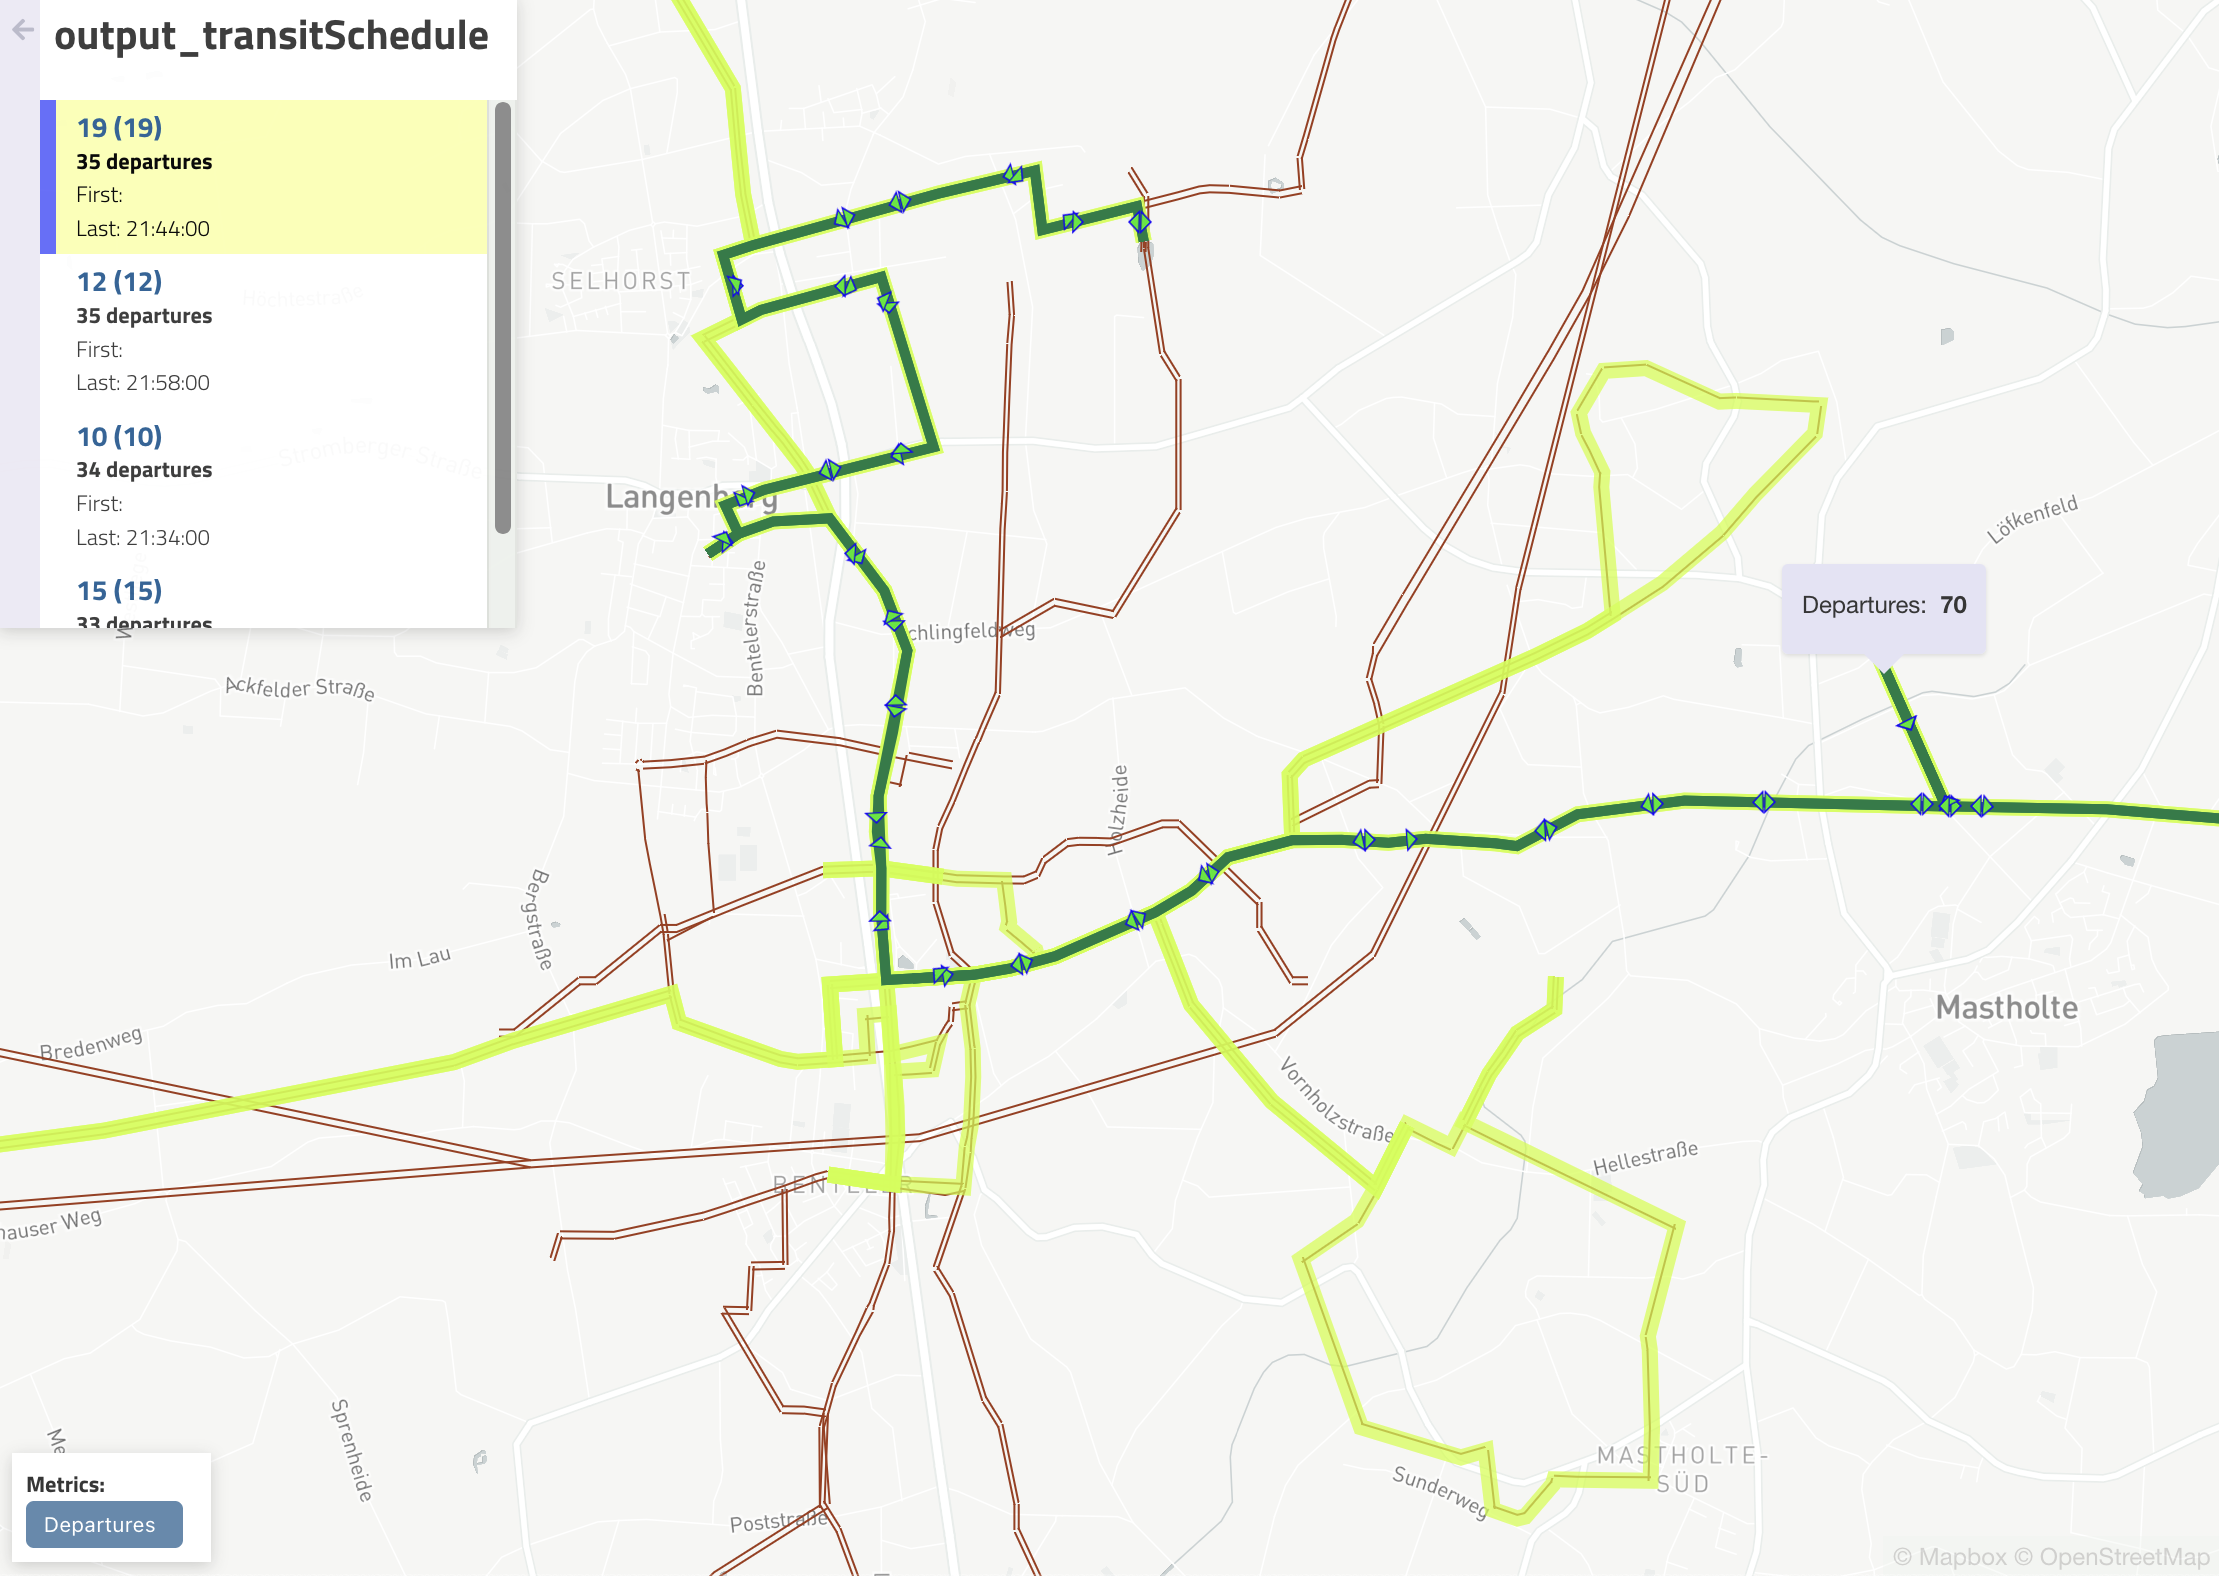
\includegraphics[width=\textwidth]{chapters/12-server-experiments/images/transit-viewer.png}
  \caption[Web-based transit network viewer]{Web-based transit network viewer. This depicts the public transit network of Cottbus, Germany, a small city in eastern Germany. One central link is selected, with the various transit routes using that line highlighted in yellow and green.}
  \label{fig:transit-viewer}
\end{figure}

As the user highlights routes in the detail view, or selects different road facilities on the map, the colors and details update immediately, allowing exploration of the transit schedule in an interactive way.

Users provided positive feedback on the tool, saying that it helped them debug network errors in complex networks, and was fast and responsive. Constructive/negative feedback highlighted initial confusion around file management and coordinate system conversion.

%% ----- GEOSERVER -----
\hypertarget{server-experiments-geoserver}{%
\section{Accessibility calculations using GeoServer and MATSim}\label{server-experiments-geoserver}}

MATSim can be used to calculate general accessibility measures, as described in \cite{ziemke2018accessibility}. For a project in Nairobi, Kenya, MATSim was used to generate accessibility measures for several different metrics such as access to drinking water, public school locations, and commercial opportunities. For each measure there were multiple scenarios such as current conditions, system breakdowns (such as a contaminated water source) and so on. The proliferation of combinations of measures and scenarios led to the idea of using the a server back-end to store results, along with a web-based front end to review results.

\gls{GeoServer}, as described in \cite{giannecchini2013geoserver}, is an open source server for sharing geospatial data.

\begin{displayquote}
\emph{"an Open Source application for the handling and dissemination of geospatial data. GeoServer provides the basic functionalities to create interoperable Spatial Data Infrastructure according to standards edited by the Open Geospatial Consortium (OGC)... GeoServer [can] ingest, manage, and serve both vector and raster geospatial data."}
\end{displayquote}

VSP has a departmental GeoServer installation, and the outputs of the accessibility calculations can be uploaded to it easily. Thus for this experiment, instead of a client-side JavaScript web application, a website front end was built that accessed the data on GeoServer using the GeoServer API.

\hypertarget{server-experiments-geoserver-2}{%
\subsection{Specifying the available accessibility measures using YAML}
\label{server-experiments-geoserver-2}}

GeoServer uses a long "string-id" to identify datasets. This ID is constructed from the scenario details. For example, the ID for the Kibera, Kenya OSM Live scenario, examining drinking water within 50 meters, with a specific color scale for relative differences of 0.5-3.5 units compared to the base case, has a string ID of

\emph{accessibilities:ke\_kibera\_osm\_live\_50\_drinking\_water\_walk\_0.5\_3.5}.

This is quite unreadable and technical for outward-facing website text, so the client website reads a YAML-based configuration file (see below) which maps the many run configurations to the appropriate GeoServer IDs. The various options are then exposed in the website user interface as drop-down selections, buttons, and so forth.

YAML itself is a simple text format which uses indentation and punctuation to define and group pairs of key:value configuration data. For example, \autoref{fig:geoserver-yaml} shows a snippet of a YAML configuration for drinking water in Kibera, Kenya.

\begin{figure}[!ht]
  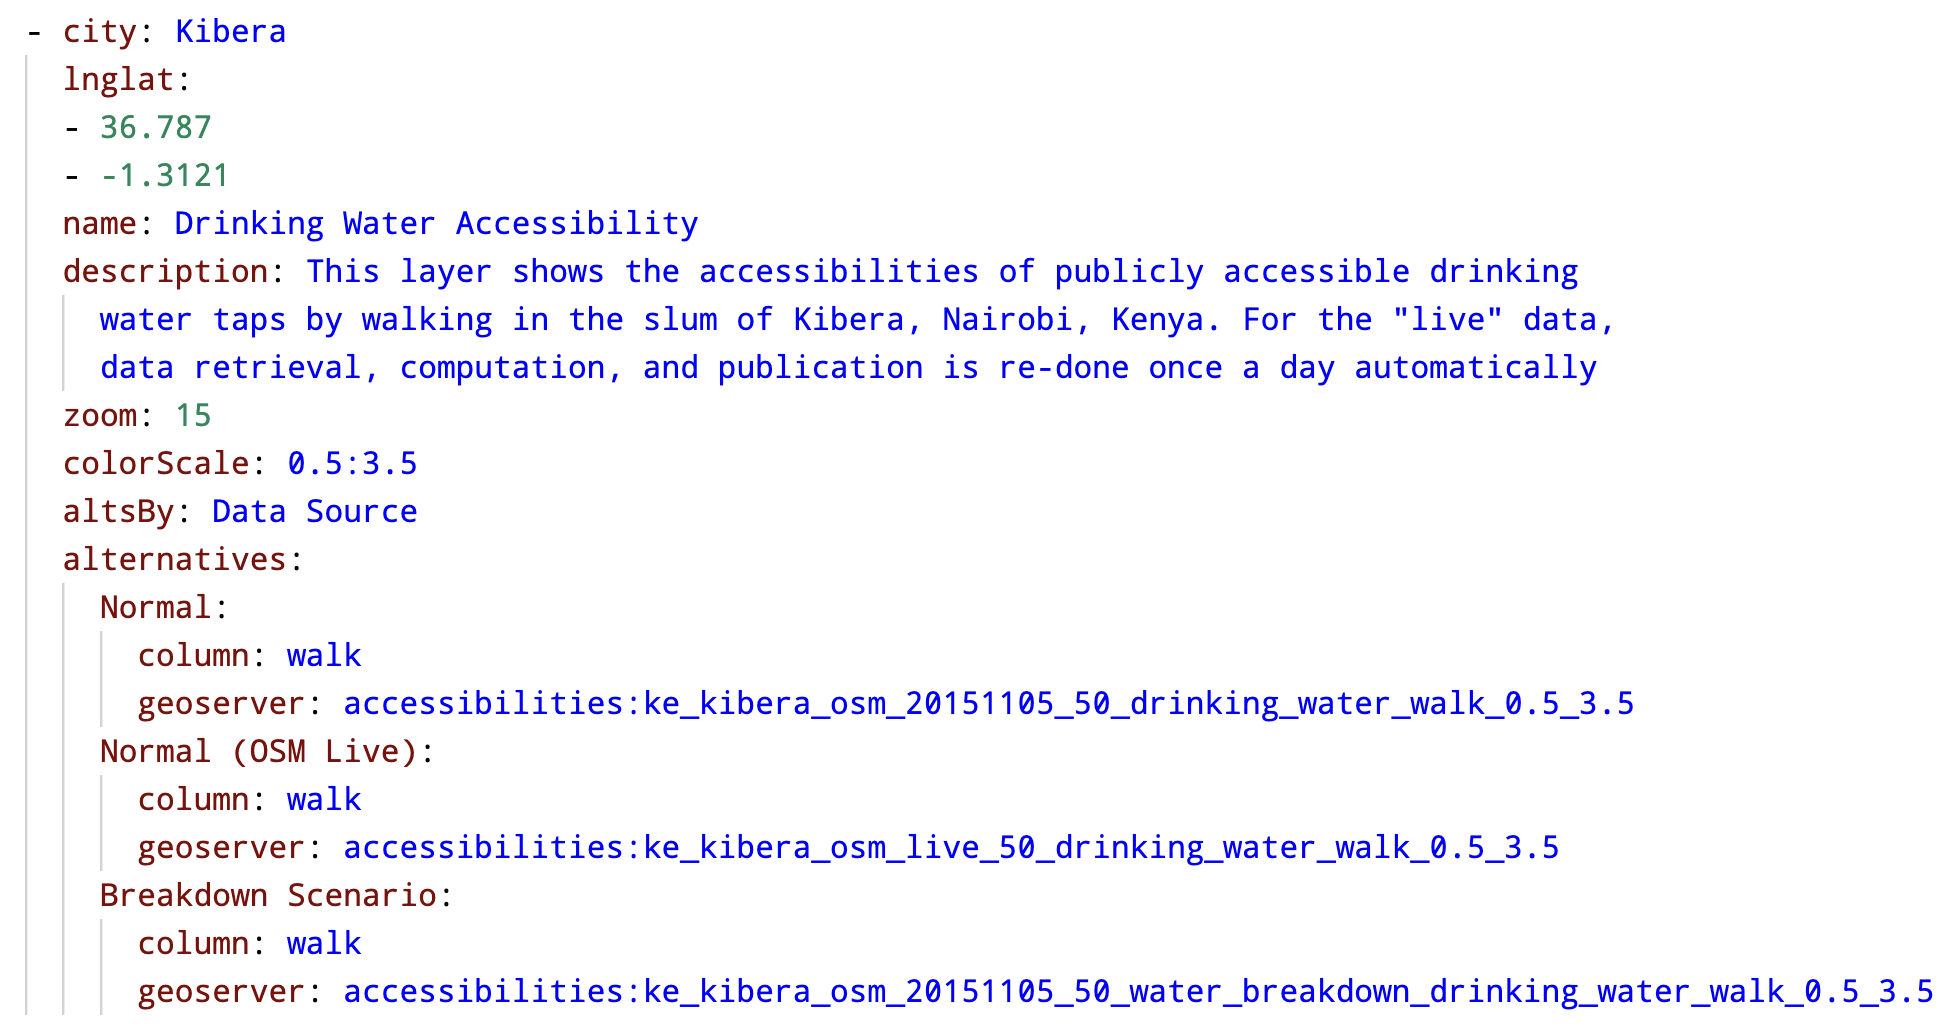
\includegraphics[width=\textwidth]{chapters/12-server-experiments/images/geoserver-yaml.png}
  \caption[GeoServer YAML configuration example]{Snippet of YAML configuration which maps user-intelligible information to GeoServer dataset IDs.}
  \label{fig:geoserver-yaml}
\end{figure}

This configuration information is read when the site is initially loaded. All of the runs defined in YAML can then be found in the user interface by selecting the metric from a dropdown and choosing the scenario for that metric with a set of buttons. The accessibility data is then pulled from the GeoServer API and displayed on top of the background map.

\hypertarget{server-experiments-geoserver-3}{%
\subsection{The Nairobi, Kenya accessibility data website}
\label{server-experiments-geoserver-3}}

\autoref{fig:nairobi} shows a typical accessibility measure displayed in the website built for the Nairobi, Kenya project. In this image, the selected metric (access to drinking water) and the scenario (normal conditions) are visible, and the grid-based accessibility values calculated by MATSim are plotted on top of the basemap. Hovering over a colored area shows the exact values for the cell in a popup hover window.

\begin{figure}[!ht]
  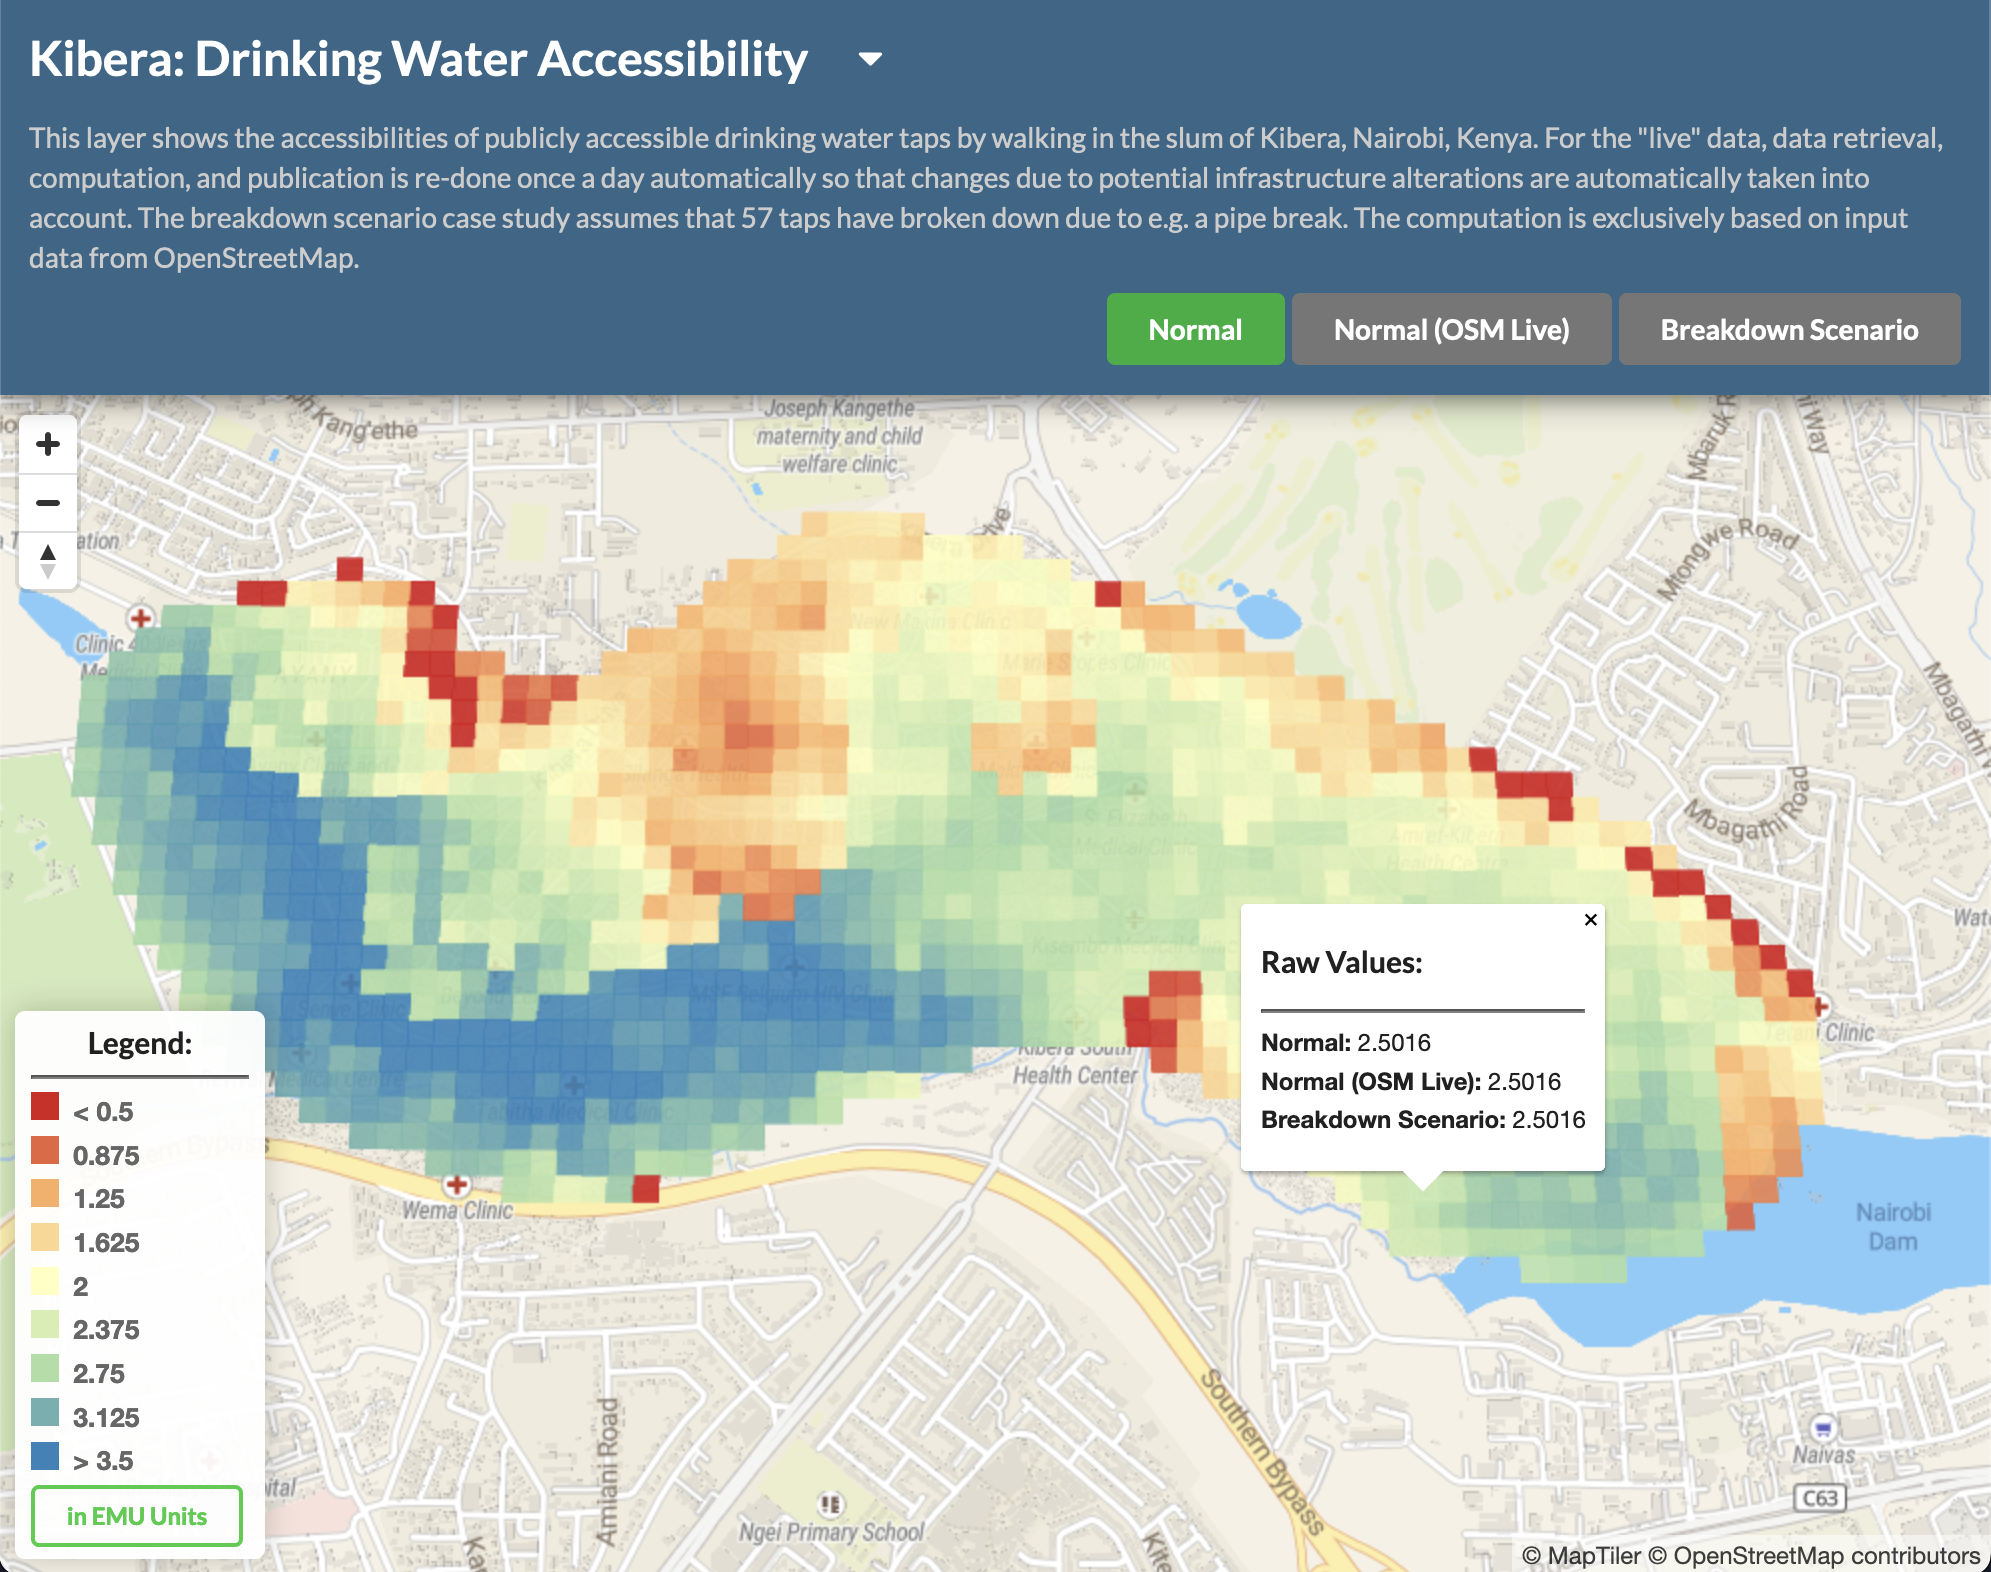
\includegraphics[width=\textwidth]{chapters/12-server-experiments/images/nairobi.png}
  \caption[Drinking water accessibility calculations, generated by MATSim]{Drinking water accessibility calculations, generated by MATSim. This interactive tool allowed users to compare accessibility calculations for drinking water, school locations, and commercial opportunities across several alternatives.}
  \label{fig:nairobi}
\end{figure}

Feedback from internal users was initially positive, as they were able to upload new runs to the server as part of their normal workflow, and updating the website only required the editing of one configuration file.

However, this approach requires manual updates from the web development team every time new data was available. For larger teams or more rapid analysis, a more streamlined and automated approach would be beneficial.

The accessibility website was not developed further after this initial project. Indeed, the GeoServer implementation at VSP was not used for any other purposes after this accessibility research concluded. Interviews revealed that department staff were unclear on the benefits of uploading their datasets to the GeoServer, when they could instead make non-interactive maps in traditional GIS desktop software, suitable for inclusion in publishable research papers.

%% ----- EMISSIONS  -----
\hypertarget{server-experiments-emissions}{%
\section{Visualizing MATSim emission outputs}
\label{server-experiments-emissions}}

MATSim emissions outputs can be derived from simulations using standard MATSim modules, as documented in \cite{Kickhoefer2015EmissionModeling}. In brief, the amount of several emission types produced on a geographic grid-cell basis are created from the standard modules and post-processing scripts output these values for each specific emission type.

As an experiment in how to ingest a large dataset by the web client and the MapBox GL visualization library, a new interactive website was custom-built for displaying MATSim emissions, with the intention to load this data in its entirety. Similar to the earlier experiments, the user can either store their simulation outputs on the departmental file server or access them via a local HTTP server running on localhost.

The size of the emission output files depends on the size of the grid cells, the number of time bins, and the geographic extent of the overall area being modeled. For the Berlin experiment, one-hour time bins and 100 meter cells resulted in individual pollutant files of approximately 150 megabytes each. Being text files, they compress by around 60-75\% -- but even so, these are rather large files to try to load into a local web browser.

It does work: after loading the data, which can take about a minute on a fast, recent laptop, the map is viewable. See \autoref{fig:emissions-grid} for an example view of emissions at the grid cell level in an area near a major freeway in Berlin.

\begin{figure}[!ht]
  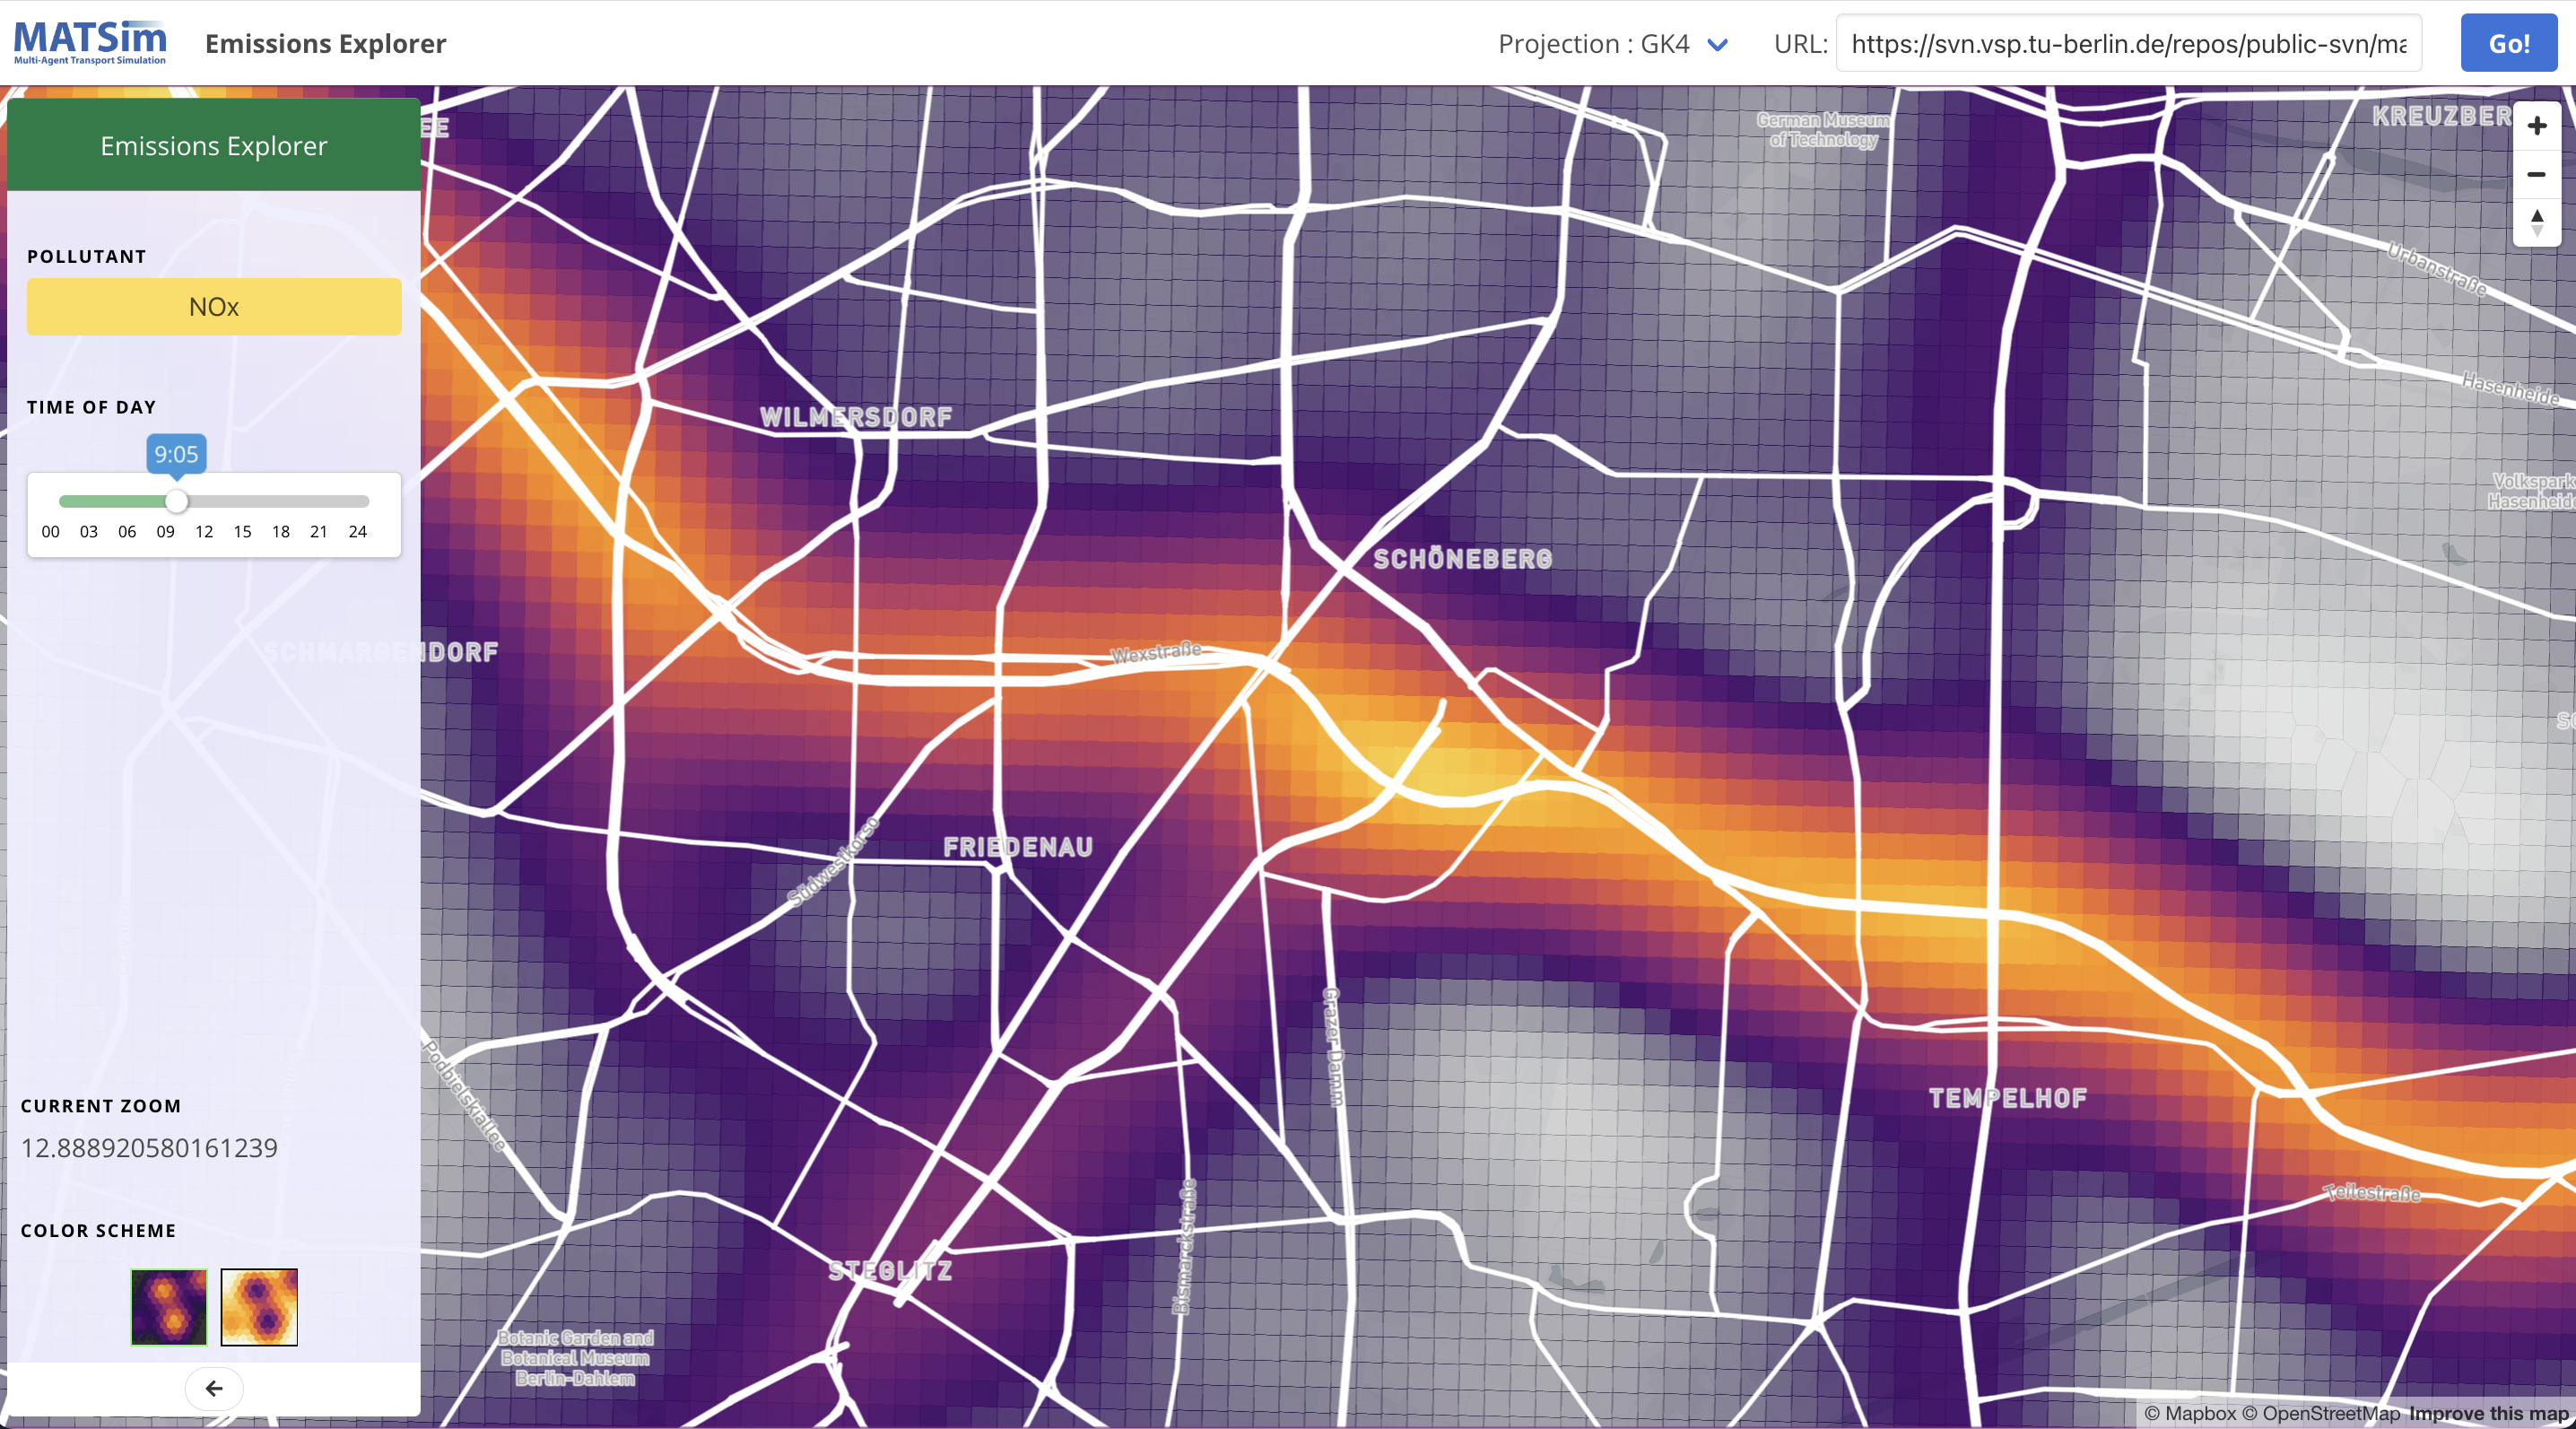
\includegraphics[width=\textwidth]{chapters/12-server-experiments/images/emissions-grid.png}
  \caption{Example grid-based emission values output by MATSim for a Berlin scenario.}
  \label{fig:emissions-grid}
\end{figure}

\hypertarget{server-experiments-emissions-lod}{%
\subsection{Level of detail}
\label{server-experiments-emissions-lod}}

A problem arises when the map is zoomed out. The MapBox GL mapping library slows down to unusable speeds when there are too many cells in the view at once. "Too many" depends on the speed of the laptop and graphics card, but the problem occurs for even the fastest laptops available for testing.

Thus, a way to trim or reduce the amount of data being displayed is necessary. Limiting the "level of detail" by selecting a subset of grid cells as the map is zoomed out successfully results in the map being viewable again. As soon as the map is zoomed, this triggers a background task that filters the dataset to the visible subset of coordinates and the values thereof.

For each of these elements, a Voronai cell is calculated which surrounds the area around the selected points. Voronai is "one of the most fundamental data structures in computational geometry" as described decades ago in \cite{aurenhammer1991voronoi} and is well-suited to this visualization type. The Voronai diagram replaces the hard, square grid of cells with variably-sized convex polygons surrounding each selected data point, so that every point on the map is inside the cell along with the closest selected point.

This approach makes for some interesting looking plots, an example of which is shown in \autoref{fig:emissions-lod}, but it also clearly warps the values being displayed. Jagged edges around the Voronai cells are especially pronounced in areas where the emissions are dropping off rapidly, such as the areas immediately adjacent to high-emission freeway segments.

\begin{figure}[!ht]
  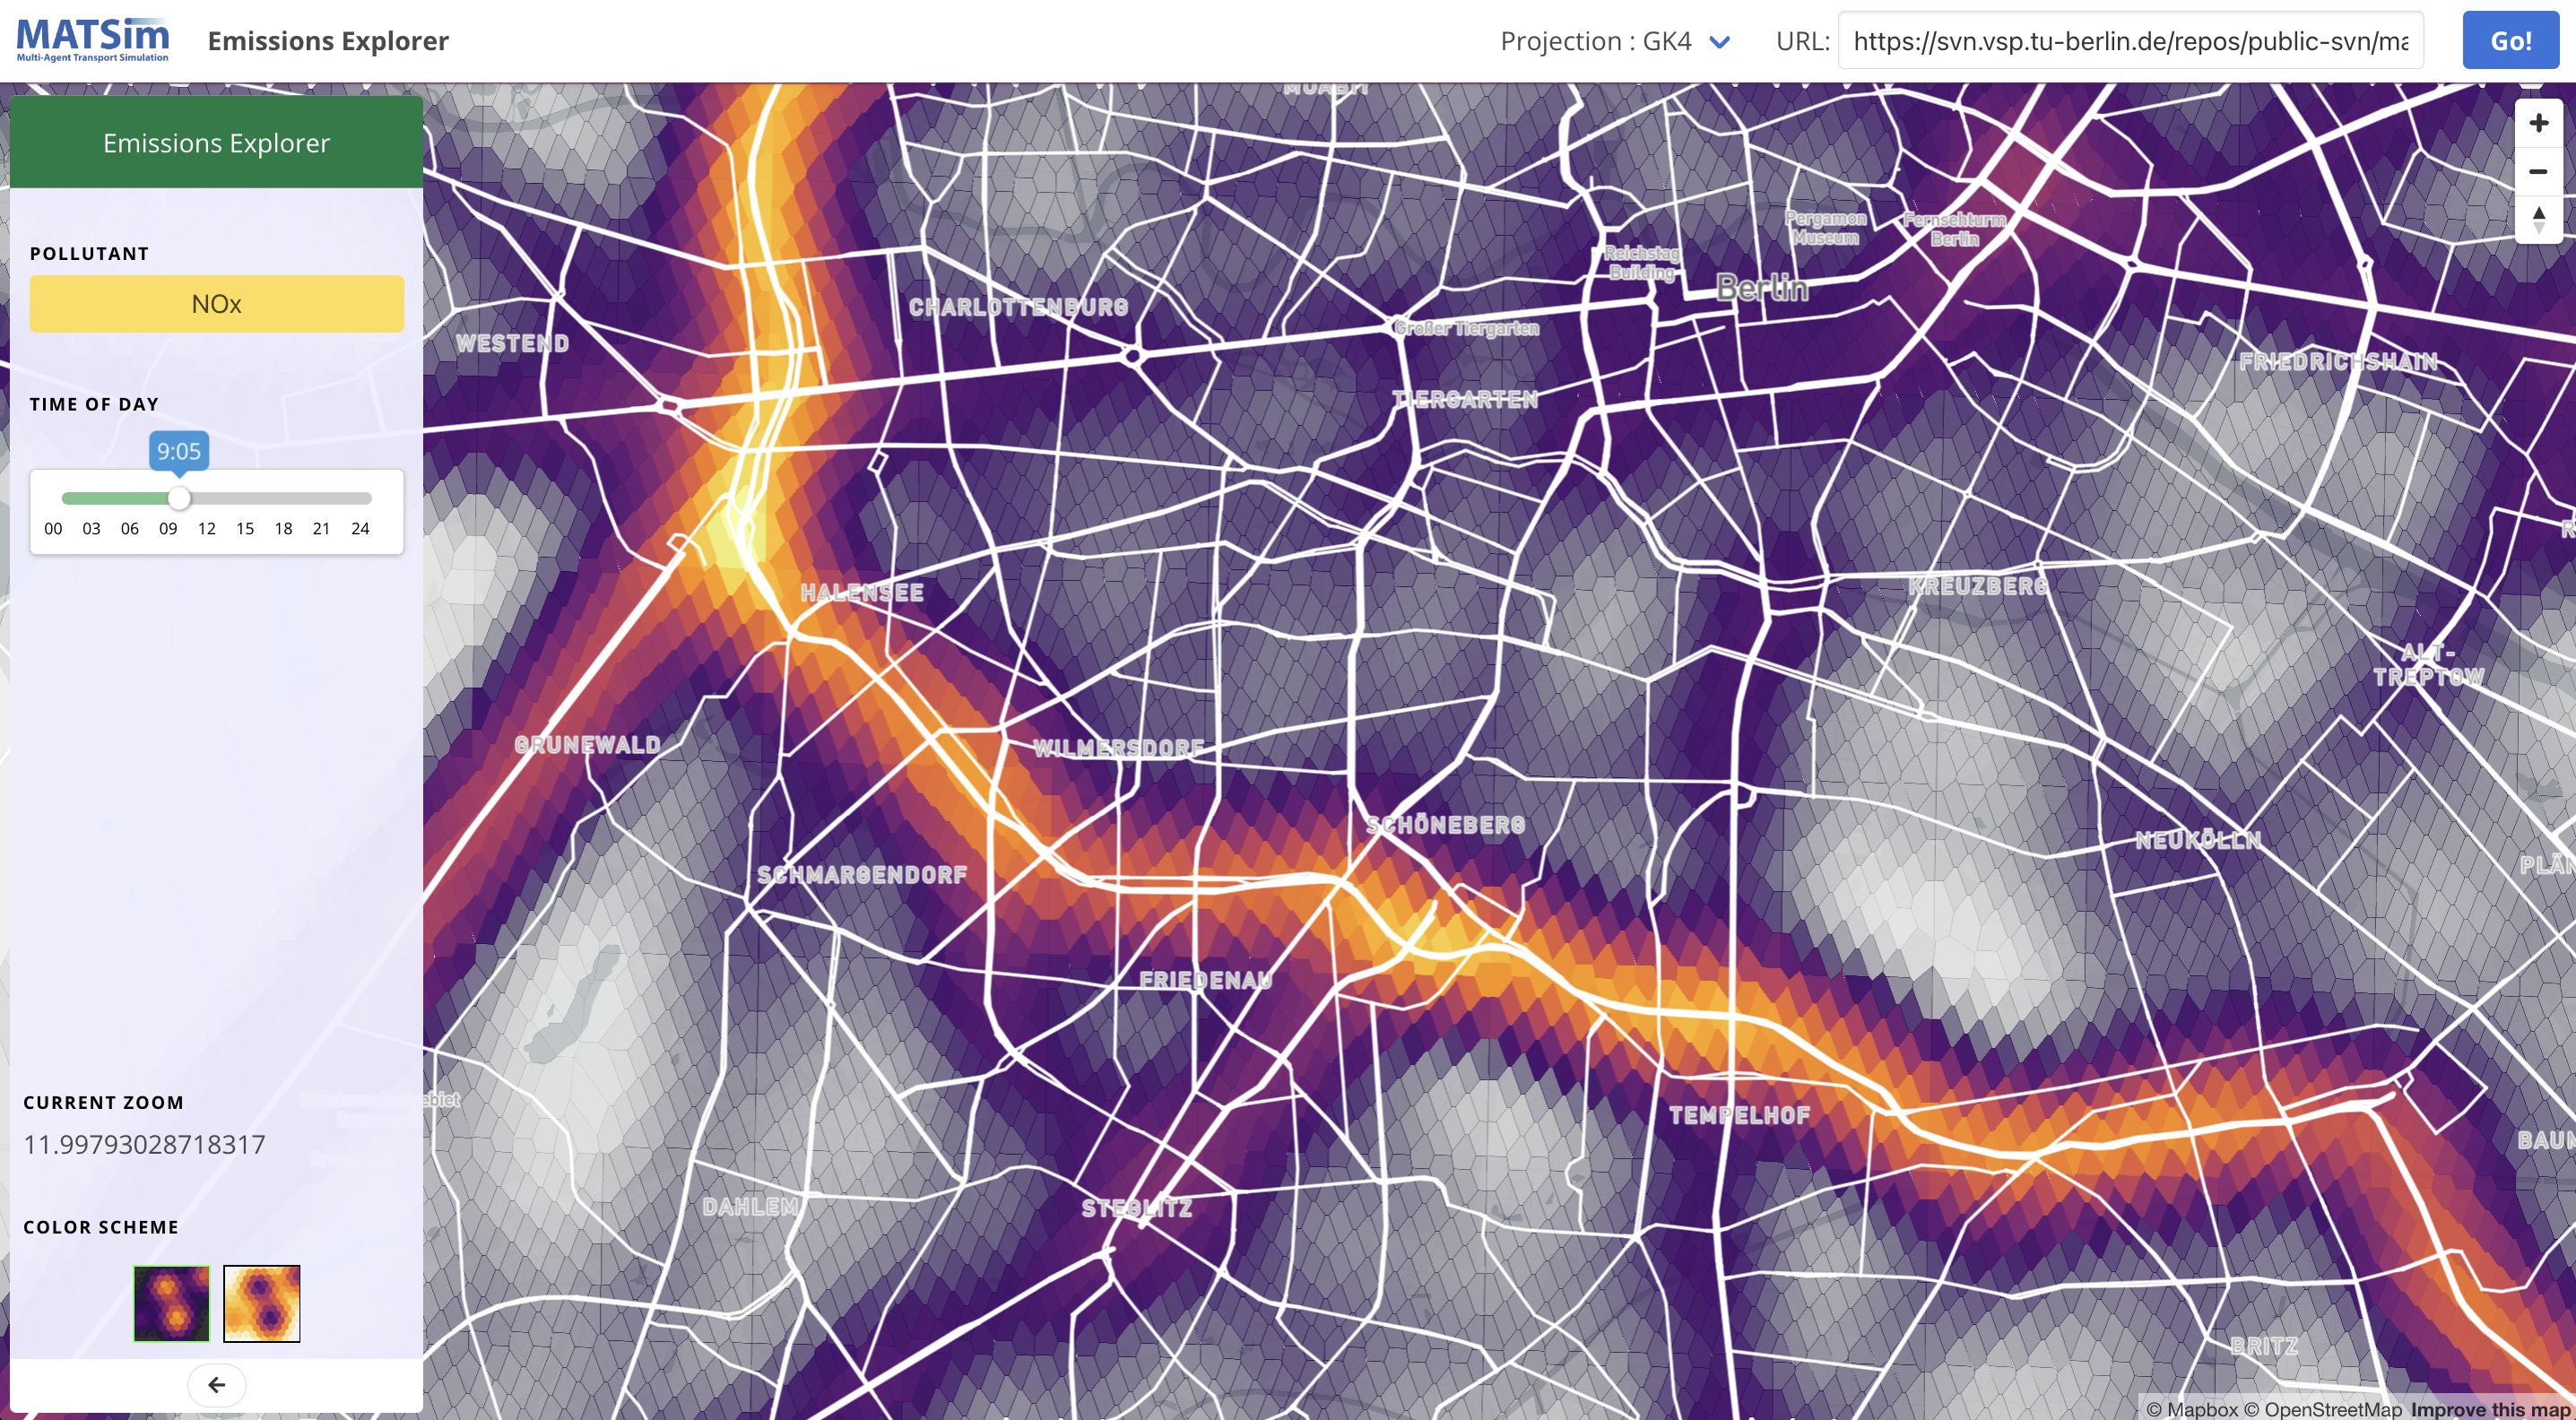
\includegraphics[width=\textwidth]{chapters/12-server-experiments/images/emissions-lod.png}
  \caption[Example Voronai areas depicting emission values for a Berlin scenario]{Example Voronai areas depicting emission values for the same Berlin scenario. This zoom level required using a level-of-detail optimization to reduce and simplify the large number of data points being drawn at the same time.}
  \label{fig:emissions-lod}
\end{figure}

The background task of calculating Voronai cells at a specified zoom level is visibly sluggish, and the results have display artifacts that may not be helpful to analysts. Between the slowness of loading the data, the sluggishness of the resulting visualization, and the compromises involved in viewing a limited level of detail at some zoom levels, this visualization experiment was not very useful for analysts at VSP.

The research on roadway emissions is published in \cite{kaddoura2022exhaust}, without reference to these visualization experiments.

%% ----- DISCUSSION AND OUTLOOK  -----
\hypertarget{server-experiments-findings}{%
\section{Discussion and Outlook}\label{server-experiments-findings}}

This set of initial experiments in using web-based technologies to visualize MATSim simulation data result in some useful findings.

First, the management of simulation output files is complex and subject to the pre-existing habits and preferences of analysts. Feedback from analysts makes it clear that MATSim outputs are almost always very large, and moving these files around from the machine they were produced on to servers for analysis or longer-term storage creates friction for analysts. That friction is high enough that very few researchers in the department are willing to try some of these features being developed for them. The alternative, running a local HTTP server to view files on a local computer, was itself also very foreign to analysts, and created another barrier to usage. Future developments must streamline the workflow and file management.

Second, there is a limit to how much data can be reasonably ingested by a local web browser. Even on the most recent and performant laptops, some datasets were simply too large to load natively and required post-processing for aggregation or pruning and filtering of datasets using "level of detail" techniques. This is a central reason why most commercially-built data analysis products rely on a back-end server which stores datasets, usually in some sort of database format, and a client front-end which displays subsets of that data as it is received. The GeoServer example above used this approach successfully. The emissions example showed the limits of the client-side approach, as the load times were unacceptable and the MapBox GL libraries could not handle the size of the datasets once loaded. (But see \autoref{ch:simwrapper} for techniques developed for successfully handling much larger datasets client-side).

Based on the results of these experiments, a client-server approach for centralizing MATSim simulation outputs and visualizations was agreed upon as a logical next step. Creating a server-backed system has some risks as noted above, but it is the approach taken by most data-heavy websites. That system is described fully in \autoref{ch:mathub}.

%% ----- SUMMARY  -----
\hypertarget{server-experiments-summary}{%
\section{Summary}\label{server-experiments-summary}}

This chapter describes a set of web-based data visualization experiments that explore different approaches to visualizing MATSim simulation outputs in various contexts.

The public transit supply viewer allows the end user to load and explore the public transit network schedule directly from the MATSim input network and transit schedule XML files. These files are small enough to be loaded directly in the browser, and users find the tool useful in debugging the transit networks for their projects.

The accessibility data tool provides an interactive, outward-facing website that depicts accessibility datasets uploaded to a central server. The tool is feature-rich, but is limited in scope to small datasets that are uploaded manually to a specific departmental server; and ultimately does not have long-term usefulness to researchers.

The emissions data experiments tested the limit of data sizes that can be ingested client-side. Files of 150 megabytes were successfully loaded, but users found the load times unacceptably slow and the operation of the website too sluggish to be useful. Smaller datasets might be more manageable, but the reality is that MATSim is used for large-scale microsimulation studies, and the size of these datasets proved too large for a fully client-side approach with the chosen JavaScript libraries and implementation.

User feedback from all of these experiments highlight the need for streamlined workflow and minimal copying of files between machines, as this creates friction for adoption.

The next chapter describes an attempt at addressing these findings in an integrated platform.
